\documentclass[french]{article}



% The default font size is 10pt; 11pt and 12pt are alternatives
%%%%%%%%%%%%%%%%%%%%%%%%%%%%%%%%%%%%%%%%%
% Professional Newsletter Template
% Structural Definitions File
% Version 1.0 (09/03/14)
%
% Created by:
% Vel (vel@latextemplates.com)
%
% This file has been downloaded from:
% http://www.LaTeXTemplates.com
%
% License:
% CC BY-NC-SA 3.0 (http://creativecommons.org/licenses/by-nc-sa/3.0/)
%
%%%%%%%%%%%%%%%%%%%%%%%%%%%%%%%%%%%%%%%%%

%----------------------------------------------------------------------------------------
%	REQUIRED PACKAGES
%----------------------------------------------------------------------------------------

\usepackage{graphicx} % Required for including images
\usepackage{microtype} % Improved typography
\usepackage{multicol} % Used for the two-column layout of the document
\usepackage{booktabs} % Required for nice horizontal rules in tables
\usepackage{wrapfig} % Required for in-line images
\usepackage{float} % Required for forcing figures not to float with the [H] parameter
\usepackage{ragged2e} 

%encoding
%--------------------------------------
\usepackage[utf8]{inputenc}
\usepackage[T1]{fontenc}
%--------------------------------------

%French-specific commands
%--------------------------------------
\usepackage[french]{babel}
\usepackage[autolanguage]{numprint}

%------------------------------------------------
%Hyphenation rules
%--------------------------------------
\usepackage{hyphenat}
\hyphenation{mathéma-tiques récu-pérer}
%--------------------------------------

% Fonts

%-\usepackage{charter} % Use the Charter font as the main document font
%-\usepackage{courier} % Use the Courier font for \texttt (monospaced) only
%-\usepackage[T1]{fontenc} % Use T1 font encoding

%------------------------------------------------
% List Separation

%-\usepackage{enumitem} % Required to customize the list environments
%-\setlist{noitemsep,nolistsep} % Remove spacing before, after and within lists for a compact look

%------------------------------------------------
% Figure and Table Caption Styles

\usepackage{caption} % Required for changing caption styles
\captionsetup[table]{labelfont={bf,sf},labelsep=period,justification=justified} % Specify the table caption style
\captionsetup[figure]{labelfont={sf,bf},labelsep=period,justification=justified, font=small} % Specify the figure caption style
\setlength{\abovecaptionskip}{10pt} % Whitespace above captions

%------------------------------------------------
% Spacing Between Paragraphs

\makeatletter
\usepackage{parskip}
\setlength{\parskip}{6pt}
\newcommand{\@minipagerestore}{\setlength{\parskip}{6pt}}
\makeatother

%----------------------------------------------------------------------------------------
%	PAGE MARGINS AND SPACINGS
%----------------------------------------------------------------------------------------

\textwidth = 7 in % Text width
\textheight = 10 in % Text height
\oddsidemargin = -18pt % Left side margin on odd pages
\evensidemargin = -18pt % Left side margin on even pages
\topmargin = -36pt % Top margin
\headheight = 0pt % Remove the header by setting its space to 0
\headsep = 0pt % Remove the space between the header and top of the page
\parskip = 4pt % Space between paragraph
\parindent = 0.0in % Paragraph indentation
\pagestyle{empty} % Disable page numbering

%----------------------------------------------------------------------------------------
%	COLORS
%----------------------------------------------------------------------------------------

\usepackage[dvipsnames,svgnames]{xcolor} % Required to specify custom colors

\definecolor{altncolor}{rgb}{.8,0,0} % Dark red
%\definecolor{altncolor}{rgb}{.2,.4,.8} % Dark blue
%\definecolor{altncolor}{rgb}{.84,.16,.16} % Red

\usepackage[colorlinks=true, linkcolor=altncolor, anchorcolor=altncolor, citecolor=altncolor, filecolor=altncolor, menucolor=altncolor, urlcolor=altncolor]{hyperref} % Use the color defined above for all links

%----------------------------------------------------------------------------------------
%	BOX STYLES
%----------------------------------------------------------------------------------------

\usepackage[framemethod=TikZ]{mdframed}% Required for creating boxes
\mdfdefinestyle{sidebar}{
    linecolor=black, % Outer line color
    outerlinewidth=0.5pt, % Outer line width
    roundcorner=0pt, % Amount of corner rounding
    innertopmargin=10pt, % Top margin
    innerbottommargin=10pt, % Bottom margin
    innerrightmargin=10pt, % Right margin
    innerleftmargin=10pt, % Left margin
    backgroundcolor=white, % Box background color
    frametitlebackgroundcolor=white, % Title background color
    frametitlerule=false, % Title rule - true or false
    frametitlerulecolor=white, % Title rule color
    frametitlerulewidth=0.5pt, % Title rule width
    frametitlefont=\Large, % Title heading font specification
    font=\small
}

\mdfdefinestyle{intextbox}{
    linecolor=black, % Outer line color
    outerlinewidth=0.5pt, % Outer line width
    roundcorner=10pt, % Amount of corner rounding
    innertopmargin=7pt, % Top margin
    innerbottommargin=7pt, % Bottom margin
    innerrightmargin=7pt, % Right margin
    innerleftmargin=7pt, % Left margin
    backgroundcolor=white, % Box background color
    frametitlebackgroundcolor=white, % Title background color
    frametitlerule=false, % Title rule - true or false
    frametitlerulecolor=white, % Title rule color
    frametitlerulewidth=0.5pt, % Title rule width
    frametitlefont=\Large % Title heading font specification
}

%----------------------------------------------------------------------------------------
%	HEADING STYLE
%----------------------------------------------------------------------------------------

\newcommand{\heading}[2]{ % Define the \heading command
\vspace{#2} % White space above the heading
{\begin{center}\Large\textbf{#1}\end{center}} % The heading style
\vspace{#2} % White space below the heading
}

\newcommand{\BackToContents}{\hyperlink{contents}{{\small Back to Contents}}} % Define a command for linking back to the contents of the newsletter






%%% ---------------
%%% DEFINITIONS
%%% ---------------

% Define separators
\newcommand{\HorRule}[1]{\noindent\rule{\linewidth}{#1}} % Creating a horizontal rule
\newcommand{\SepRule}{\noindent							 % Creating a separator
						\begin{center}
							\rule{250pt}{1pt}
						\end{center}
						}

% Define Title en News input
\newcommand{\JournalName}[1]{%
		\begin{center}
			\Huge \usefont{T1}{QTCaligulatype}{m}{n}
			#1%
		\end{center}
		\par \normalsize \normalfont}

\newcommand{\JournalIssue}[1]{%
		\hfill \textsc{\mydate \today, No #1}
		\par \normalsize \normalfont}

\newcommand{\NewsItem}[1]{%
		\usefont{T1}{augie}{m}{n}
		\large #1 \vspace{4pt}
		\par \normalsize \normalfont}

\newcommand{\NewsAuthor}[1]{%
			\hfill by \textsc{#1} \vspace{4pt}
			\par \normalfont}
 % Include the document which specifies all packages and structural customizations for this template

\begin{document}


%----------------------------------------------------------------------------------------
%	HEADER IMAGE
%----------------------------------------------------------------------------------------

% Title
% -----
\JournalName{\Huge\textbf {LETTRE D'INFORMATION SUR LES AMENDES RGPD  }}
\noindent\HorRule{3pt} \\[-0.75\baselineskip]
\HorRule{1pt}

\vspace{0.5cm}
	\SepRule
\vspace{0.5cm}


%General Statistic
\NewsItem{\raggedright{\LARGE Amendes RGPD Sanctionnées en résumé}}
\justify
Le règlement nᵒ 2016/679, dit règlement général sur la protection des données, est un règlement de l'Union européenne qui constitue le texte de référence en matière de protection des données à caractère personnel. \\
\textbf{530} des amendes ont été infligées jusqu'à aujourd'hui.
Le total cumulé des amendes pour la protection des données s'élève désormais à \textbf{275 187 314€}.


\begin{figure}
	[H]\centering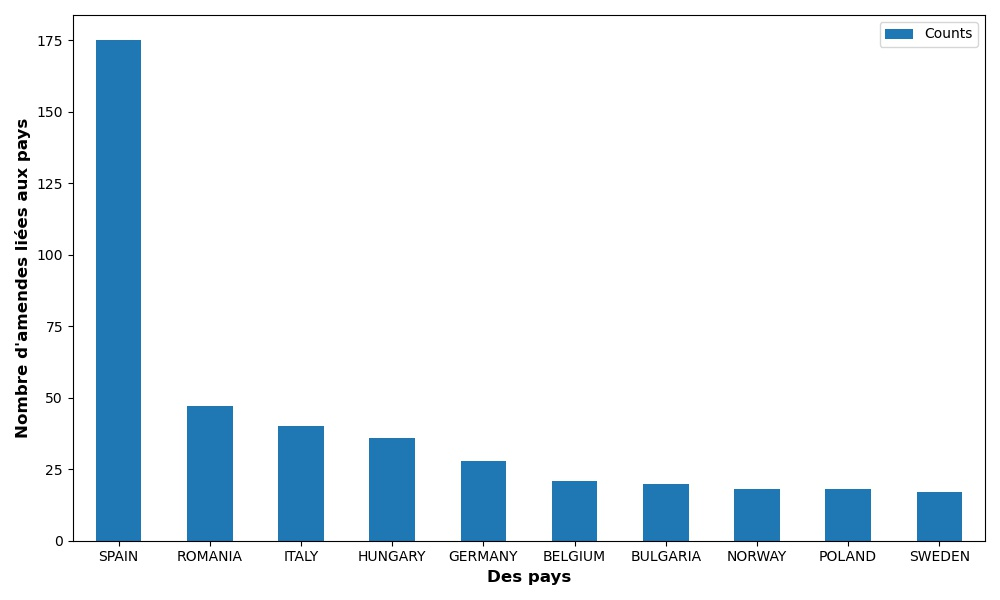
\includegraphics[width=0.7\linewidth]{graphs/top10_countries}
      \caption{Top 10 des pays de l'UE avec le plus grand nombre d'amendes}
\end{figure}
\begin{figure}
	[H]\centering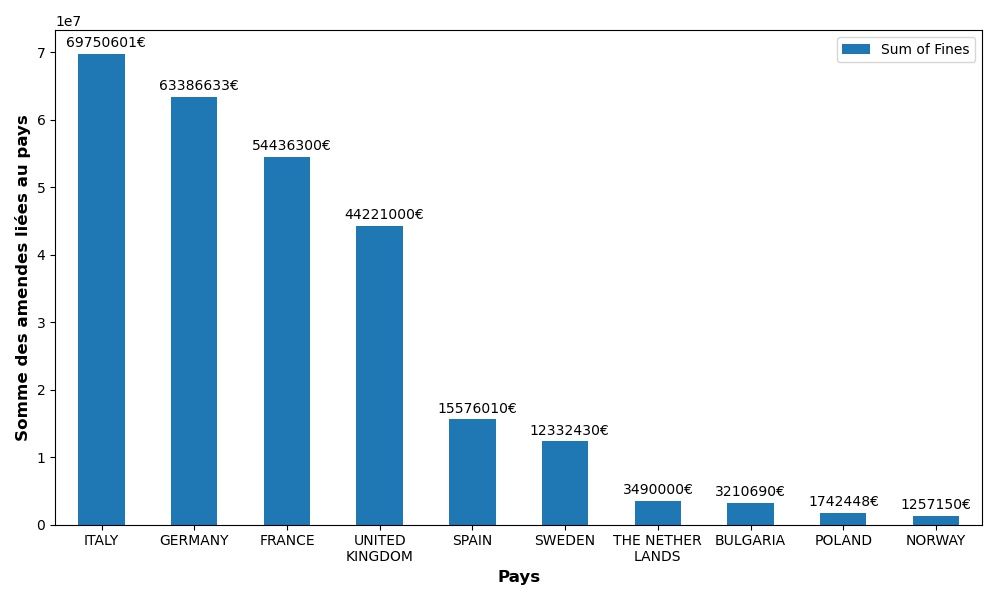
\includegraphics[width=0.7\linewidth]{graphs/top10_countries_fines}
	\caption{Top 10 des pays de l'UE avec la somme d'amendes la plus élevée}
 \end{figure}


\newpage

	\begin{multicols}{2}
	\begin{figure}
		[H]\centering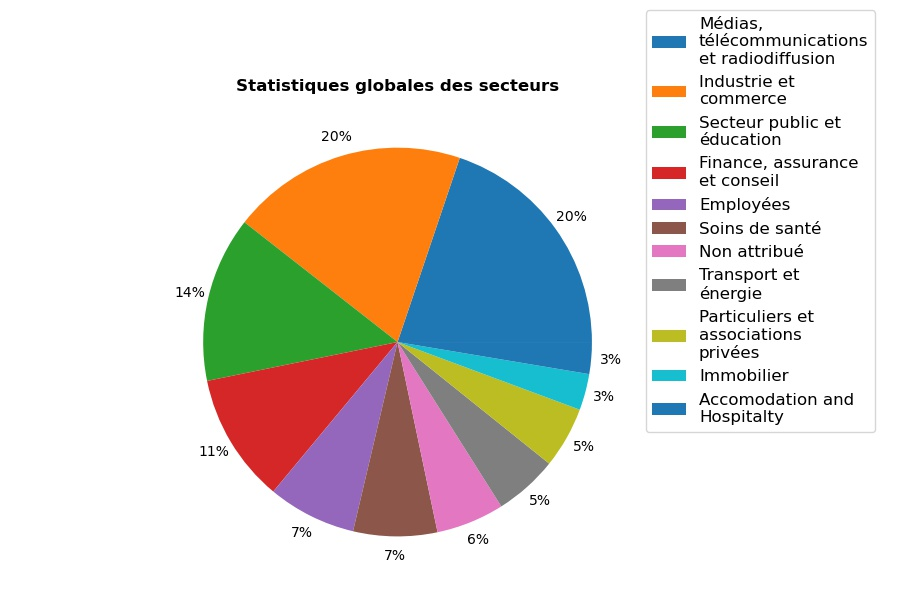
\includegraphics[width=1.0\linewidth]{graphs/sector_data}
		\caption{Top 10 des secteurs avec le plus grand nombre d'amendes}
	\end{figure}
	\begin{figure}
		[H]\centering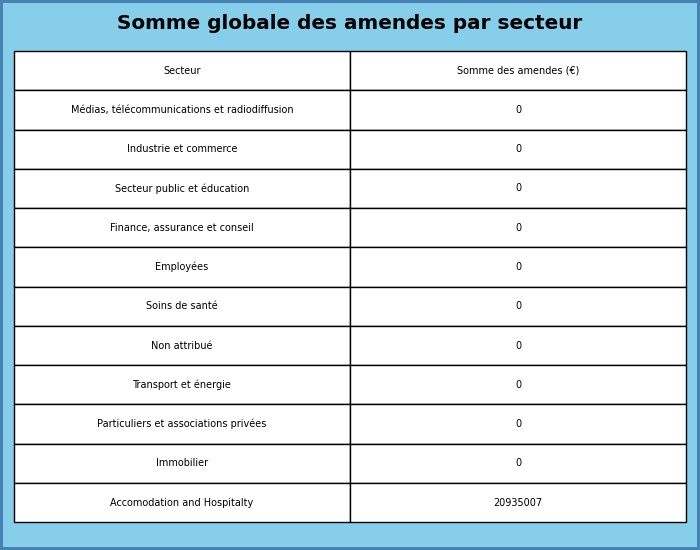
\includegraphics[width=1\linewidth]{graphs/sector_data_fines}
		\caption{Top 10 des entreprises avec le plus grand nombre d'amendes}
	 \end{figure}
	
	\end{multicols}
	
	
	
	\begin{figure}
		[H]\centering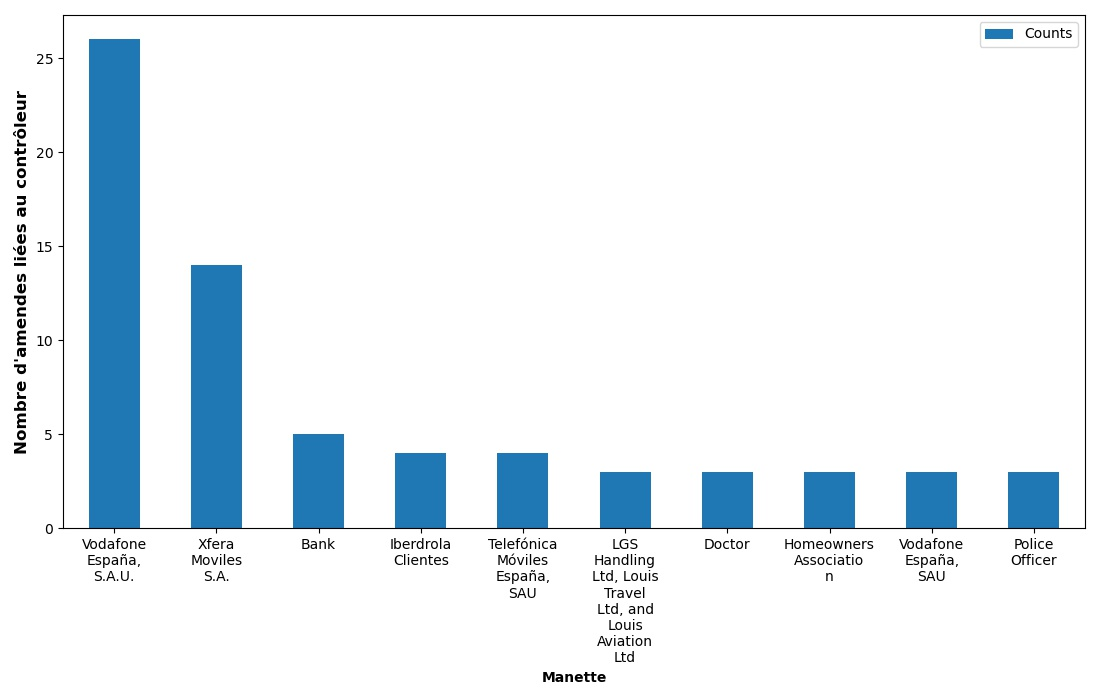
\includegraphics[width=0.6\linewidth]{graphs/top10_controller}
		\caption{Top 10 des entreprises avec le plus grand nombre d'amendes}
	\end{figure}
	
	\begin{figure}
		[H]\centering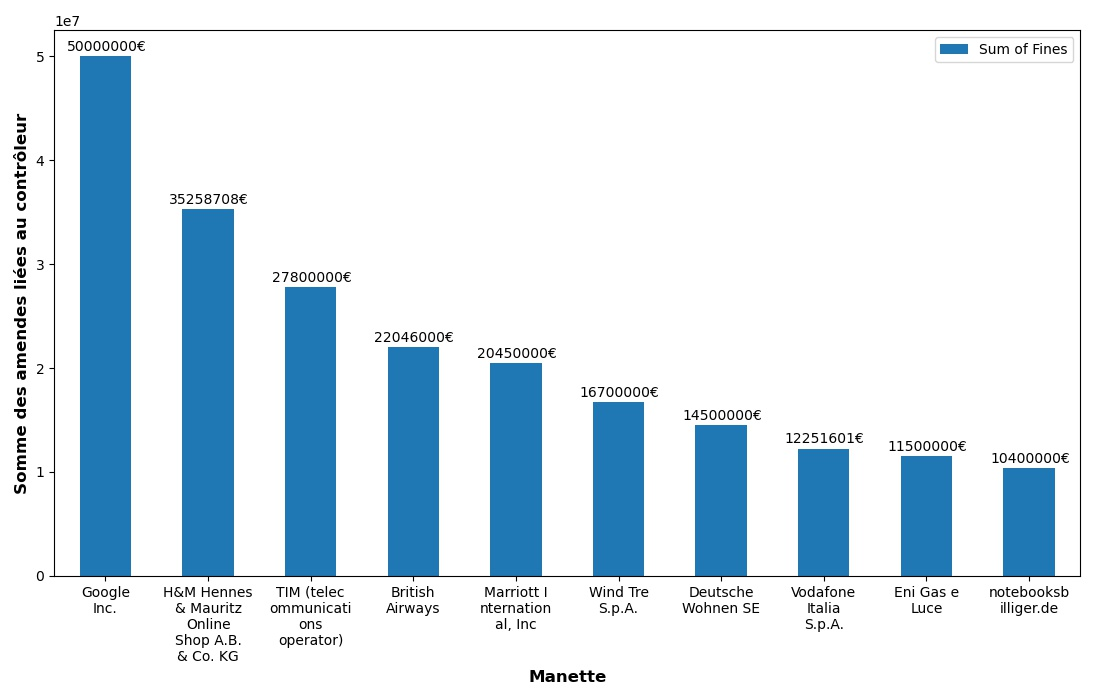
\includegraphics[width=0.6\linewidth]{graphs/top10_controller_fines}
		\caption{Top 10 des entreprises avec le montant le plus élevé d'amendes}
	 \end{figure}



\newpage


	\begin{multicols}{2}
	\begin{figure}
		[H]\centering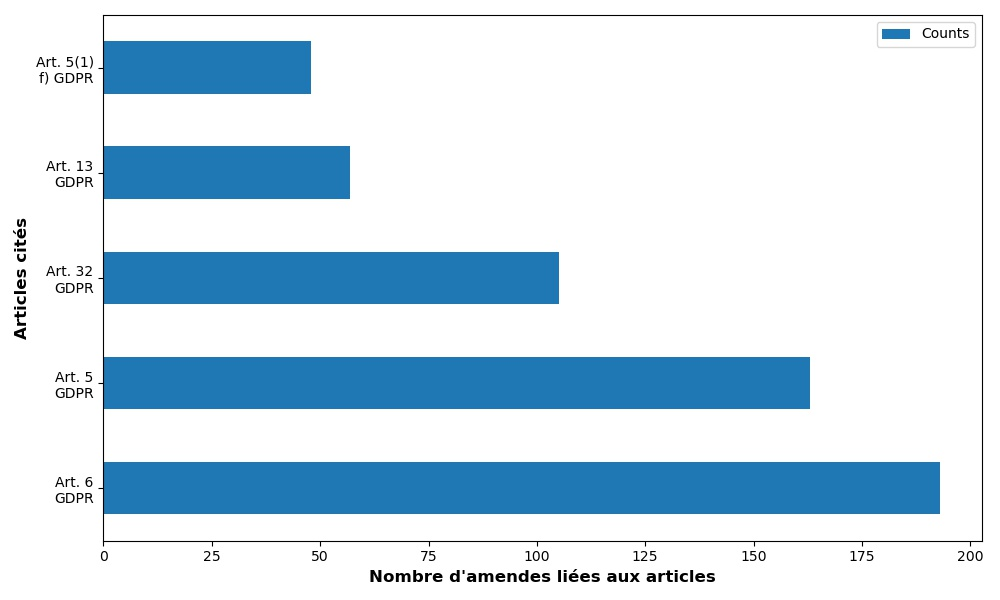
\includegraphics[width=1\linewidth]{graphs/top10_quoted} 
		\caption{Top 5 des articles cités du RGPD avec le plus grand nombre d'amendes}
	\end{figure}
	\begin{figure}
		[H]\centering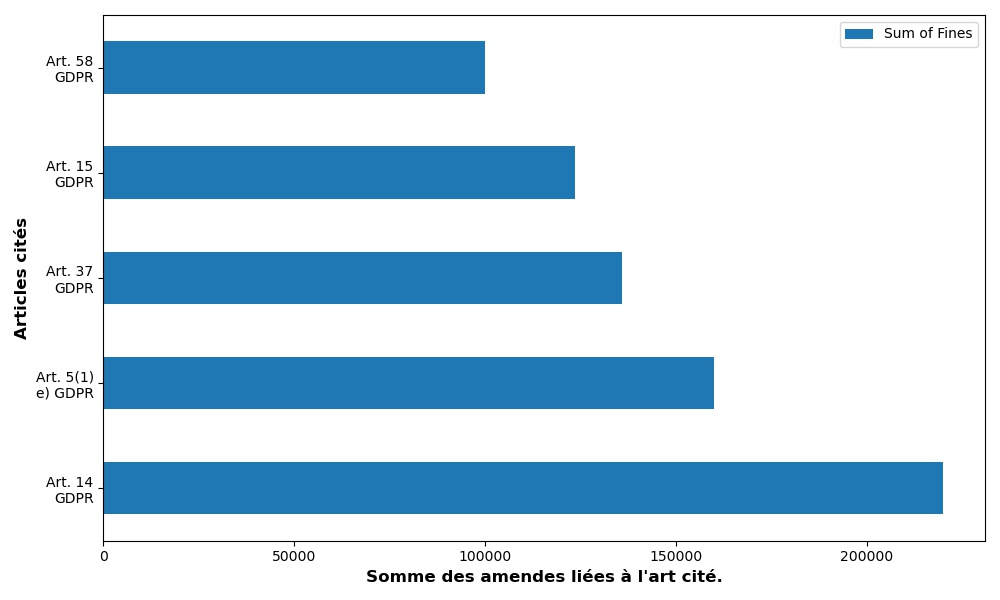
\includegraphics[width=1\linewidth]{graphs/top10_quoted_fines} 
		\caption{Top 5 des articles  du RGPD avec le montant le plus élevé d'amendes}
	\end{figure}
	\end{multicols}
	
	
	\NewsItem{\raggedright{\LARGE Analyse sur l'application du RGPD au fil des ans}}
	\begin{figure}
		[H]\centering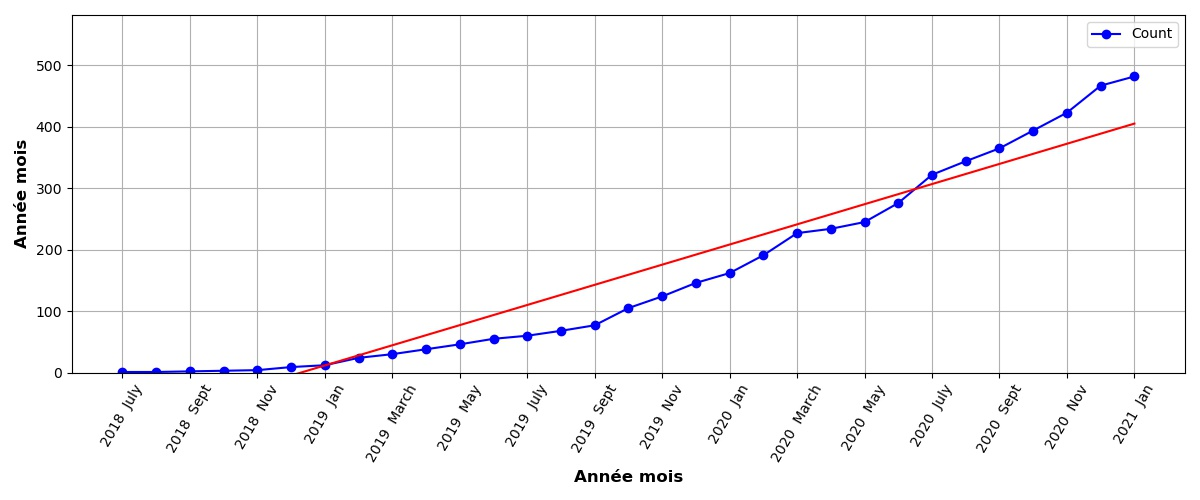
\includegraphics[width=0.8\linewidth]{graphs/acc_nb_cases_graph}
		\caption{Le nombre d'amendes (cumulatif) }
	\end{figure}
	
	\begin{multicols}{2}
	\begin{figure}
		[H]\centering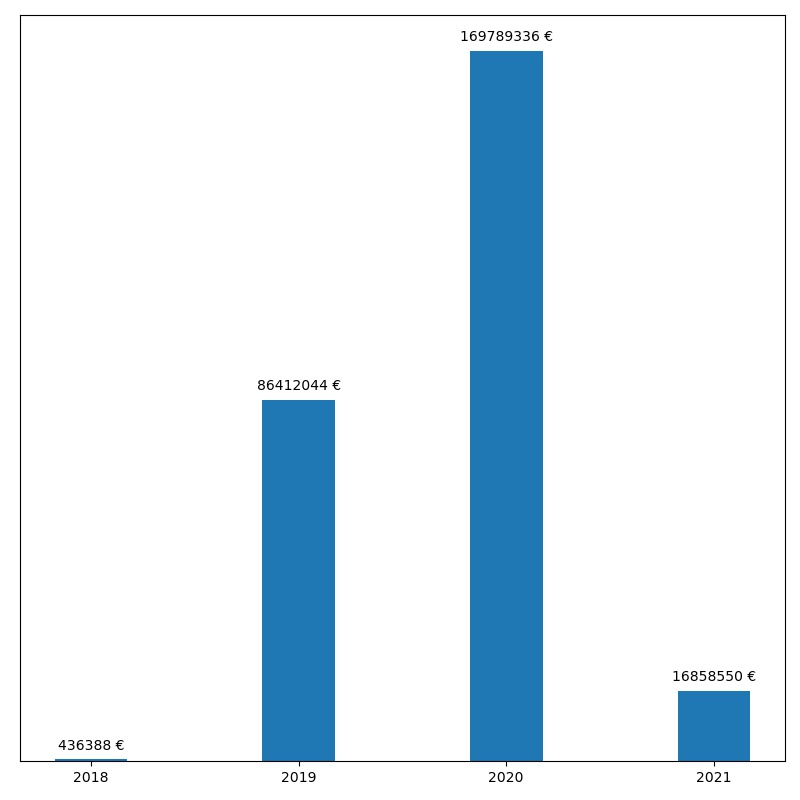
\includegraphics[width=1.0\linewidth]{graphs/SumOfFinesperYear}
		\caption{La somme d'amende par an }
	 \end{figure}
\justify
	L'application du RGPD s'est accélérée depuis les premières années, tant sur le nombre de cas d'exécution que sur la somme des amendes. La sensibilisation du public et la couverture médiatique de la vie privée et de la protection des données se sont également accrues au fil des ans. Cependant, le RGPD risque d'échouer. Selon une étude de Brave, cela est dû au fait que les autorités de protection des données (DPA) ne donnent pas suffisamment de ressources humaines et financières pour accomplir leurs tâches. Seuls 6 DPA nationaux disposent de plus de 10 enquêteurs techniques spécialisés. La moitié de toutes les APD nationales reçoivent de petits budgets annuels (5 millions d'euros ou moins) de leurs gouvernements.
	\end{multicols}



\newpage



%Particular Year Statistic
\NewsItem{\raggedright{\LARGE Amendes RGPD Sanctionnées en 2020}}

	\begin{multicols}{2}
	
	En 2020,  il y a eu \textbf{321} amendes.
	Le total cumulé des amendes de protection des données pour 2020 se tient maintenant à \textbf{169 789 336€}.
	
	\begin{figure}[H]
	\centering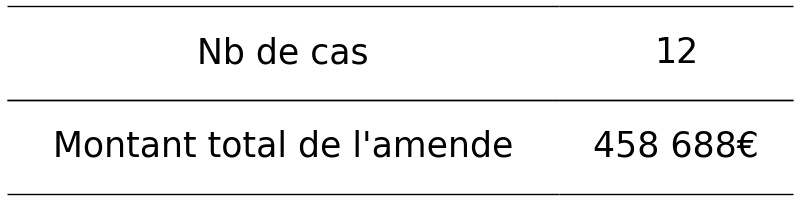
\includegraphics[width=1\linewidth]{graphs/counter_year}
	\end{figure}


	Les amendes du RGPD pour 2020 se résume pour chaque mois comme suit :

	\begin{figure}
	[H]\centering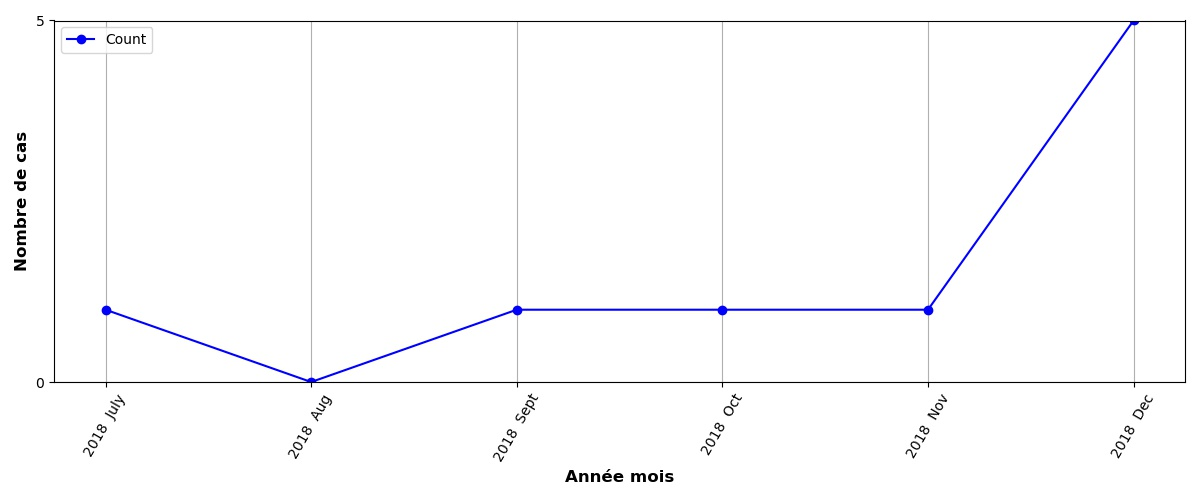
\includegraphics[width = 1.2\linewidth]{graphs/NbFinesPerMonth_year_graph}
	\caption{Petit aperçu sur des mois 2020}
	\end{figure}

	\end{multicols}


	\begin{figure}
		[H]\centering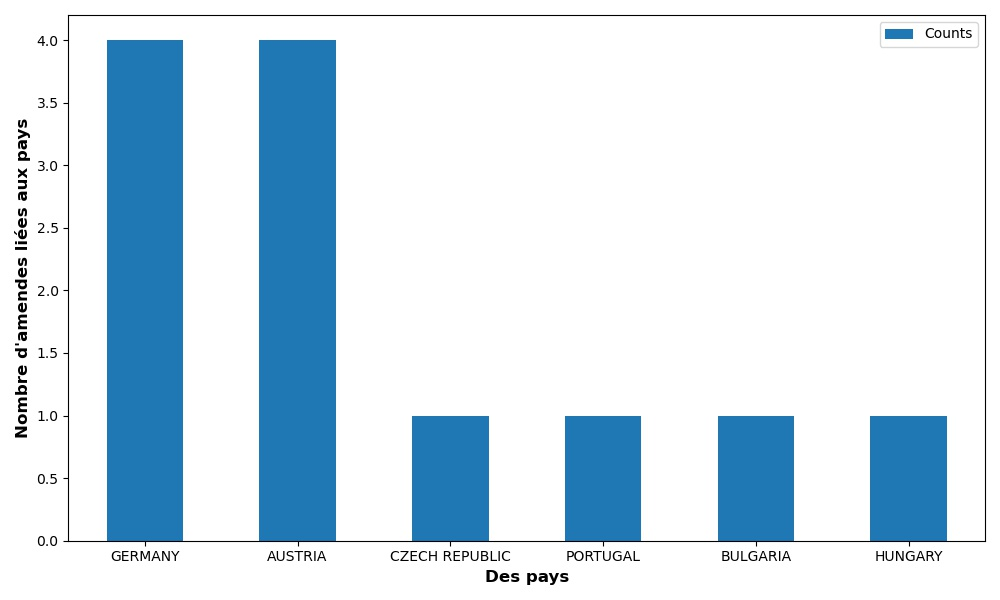
\includegraphics[scale=.5]{graphs/top10_countries_year}
		\caption{Top 10 des pays de l'UE avec le plus grand nombre d'amendes en 2020}
	\end{figure}
	\begin{figure}
		[H]\centering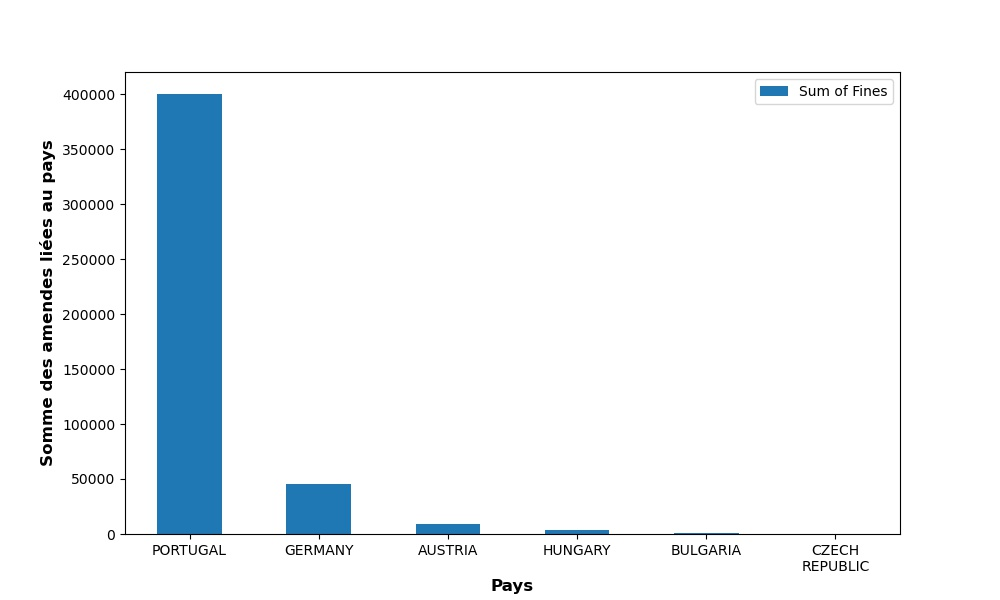
\includegraphics[scale=.5]{graphs/top10_countries_year_fines}
		\caption{Top 10 des pays de l'UE avec la somme d'amendes la plus élevée en 2020}
	\end{figure}

\newpage
\justify
	\begin{multicols}{2}
	\heading{3 amendes les plus récentes en 2020}{3 pt}
		\begin{itemize}
			\item \textbf{2020-12-30} \newline
			3,000€ d'amende en ROUMANIE pour ING Bank N.V. Amsterdam - Bureau de Bucarest.
			\newline
			La DPA roumaine (ANSPDCP) a infligé une amende de 3 000 EUR à l'agence ING Bank N.V. Amsterdam - Bucarest.
			\newline
			\href{https://www.dataprotection.ro/?page=Comunicat_presa_30_12_2020&lang=ro}{Plus d'informations}
			\vspace{1cm}
	
			\item \textbf{2020-12-29} \newline
			1,000€ d'amende en ROUMANIE pour Qualitance QBS SA.
			\newline
			La DPA roumaine (ANSPDCP) a condamné Qualitance QBS SA à une amende de 1 000 EUR pour violation de l'art.
			\newline
			\href{https://www.dataprotection.ro/?page=Comunicat_Presa_29_12_2020&lang=ro}{Plus d'informations}
			\vspace{1cm}
	
			\item \textbf{2020-12-28} \newline 18,930€ d'amende en POLOGNE pour Towarzystwo Ubezpieczeń i Reasekuracji WARTA S.A.
			\newline
			La DPA polonaise (UODO) a condamné Towarzystwo Ubezpieczeń i Reasekuracji WARTA S.A. à une amende de 18 930 EUR pour violation de l'art. 33 (1) RGPD et art. 34 (1) du RGPD.En mai 2020, la DPA a reçu une notification d'un tiers concernant une violation de données personnelles impliquant un agent d'assurance agissant en tant qu'agent de traitement pour Towarzystwo Ubezpieczeń i Reasekuracji WARTA S.A. qui a envoyé une police d'assurance à un destinataire non autorisé par courrier électronique. Le document contenait des données personnelles concernant, entre autres, les noms, prénoms, adresses résidentielles et des informations au sujet de la police d'assurance.En conséquence, l'autorité de contrôle a demandé au responsable du traitement de clarifier si, concernant l'envoi de la correspondance électronique à un destinataire non autorisé, une analyse des risques sur la sécurité des données des personnes physiques avait été effectuée, ce qui est nécessaire pour évaluer si une violation de données s'était produit. Une telle violation nécessite une notification à l'APD et aux personnes concernées par la violation. Dans la lettre, l'autorité de contrôle a indiqué au responsable du traitement comment notifier la violation et a demandé des explications.Malgré la lettre demandant des explications, le responsable du traitement n'a pas signalé la violation de données ni informé les personnes concernées de l'incident. La DPA a donc engagé une procédure administrative. Ce n'est qu'à la suite de l'ouverture de la procédure que le responsable du traitement a signalé la violation de données à caractère personnel et informé deux personnes concernées par la violation.
			\newline
			\href{https://uodo.gov.pl/decyzje/DKN.5131.5.2020}{Plus d'informations}
		\end{itemize}
	\end{multicols}

\newpage
\justify
	\begin{multicols}{2}
		\heading{Amendes notables en 2020}{3 pt}
		\begin{itemize}
			\item \textbf{La plus grosse amende} en 2020 - \textbf{35258708 €} a été condamné par ALLEMAGNE à Boutique en ligne Hu0026M Hennes u0026 Mauritz A.B..
			\newline
			\textbf{Résumé} : L'entreprise de mode avec siège à Hambourg exploite un centre de services à Nuremberg. Ici, selon les conclusions du délégué à la protection des données de Hambourg, depuis au moins 2014, les circonstances de la vie privée de certains employés ont été enregistrées de manière exhaustive et ces informations stockées sur un lecteur réseau. Par exemple, l'entreprise a organisé une conférence de bienvenue après le retour des employés au travail après des vacances ou une maladie. Les informations devenues connues dans ce contexte - y compris les informations sur les symptômes de maladie et les diagnostics des employés - ont été enregistrées et stockées. En outre, selon l'autorité de protection des données de Hambourg, certains superviseurs ont également utilisé le Flurfunk [c'est-à-dire entendre quelque chose à travers la vigne) pour acquérir une connaissance approfondie des employés individuels, par exemple sur les problèmes familiaux et les croyances religieuses. Les informations stockées sur le lecteur réseau étaient accessibles à un maximum de 50 dirigeants de l'entreprise et ont été utilisées, entre autres, pour évaluer le rendement au travail des employés et pour prendre des décisions d'emploi. La collecte de données est devenue connue en raison d'une erreur de configuration technique. en octobre 2019, selon lequel les données stockées sur le lecteur réseau étaient accessibles dans toute l'entreprise pendant plusieurs heures. Après que l'infraction a été connue, la direction s'est excusée auprès des employés et a offert une compensation monétaire. En outre, d'autres mesures de protection ont également été introduites en collaboration avec l'autorité de protection des données. [Remarque: la base juridique concrète de l'amende n'est pas encore publiée - nous supposons qu'il s'agira principalement de l'art. 5 et 6 RGPD)
			\newline
			\href{https://datenschutz-hamburg.de/pressemitteilungen/2020/10/2020-10-01-h-m-verfahren}{Plus d'informations}
			\vspace{1cm}
		
			\item \textbf{La plus petite amende} en 2020 - \textbf{28 €} -  a été condamné par  à Google Ireland Ltd..
			\newline
			\textbf{Résumé} : Absence de réponse à une demande d'accès aux informations (art. 15 RGPD - ici: sur les données traitées dans le cadre de Google AdWords) en temps voulu.
			\newline
			\href{https://www.naih.hu/files/NAIH-2020-5553-hatarozat.pdf}{Plus d'informations}
		\end{itemize}
	\end{multicols}


\newpage

	
	\begin{multicols}{2}
	\begin{figure}
		[H]\centering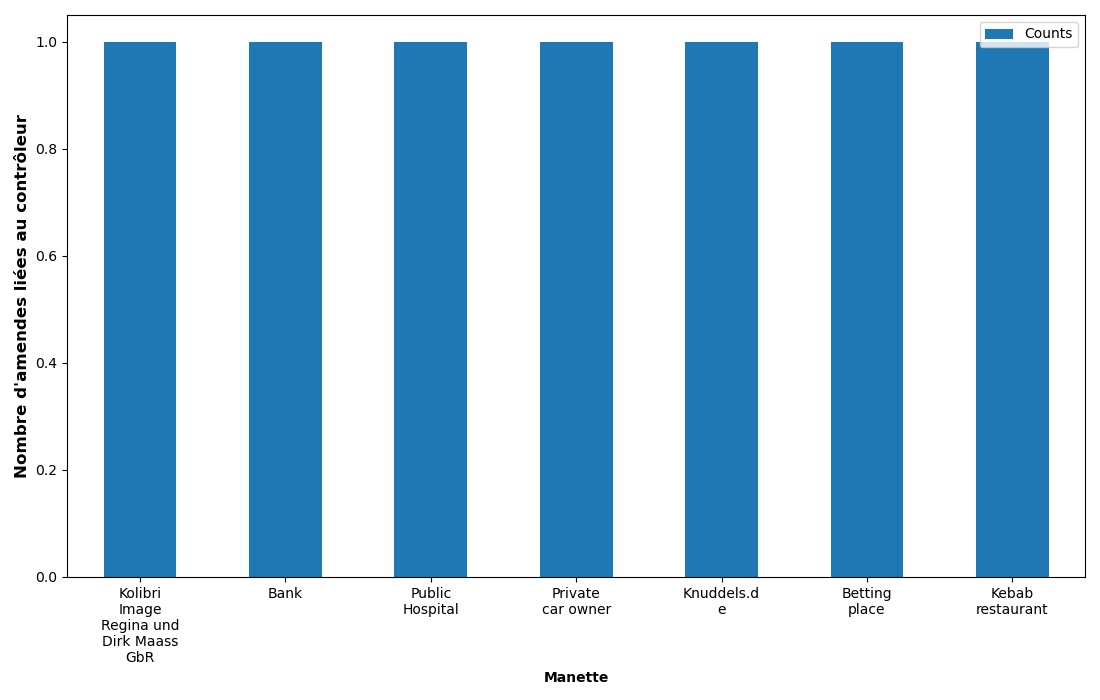
\includegraphics[width=1.0\linewidth]{graphs/top10_controller_year}
		\caption{Top 10 des entreprises avec le plus grand nombre d'amendes en2020}
	\end{figure}
	\begin{figure}
		[H]\centering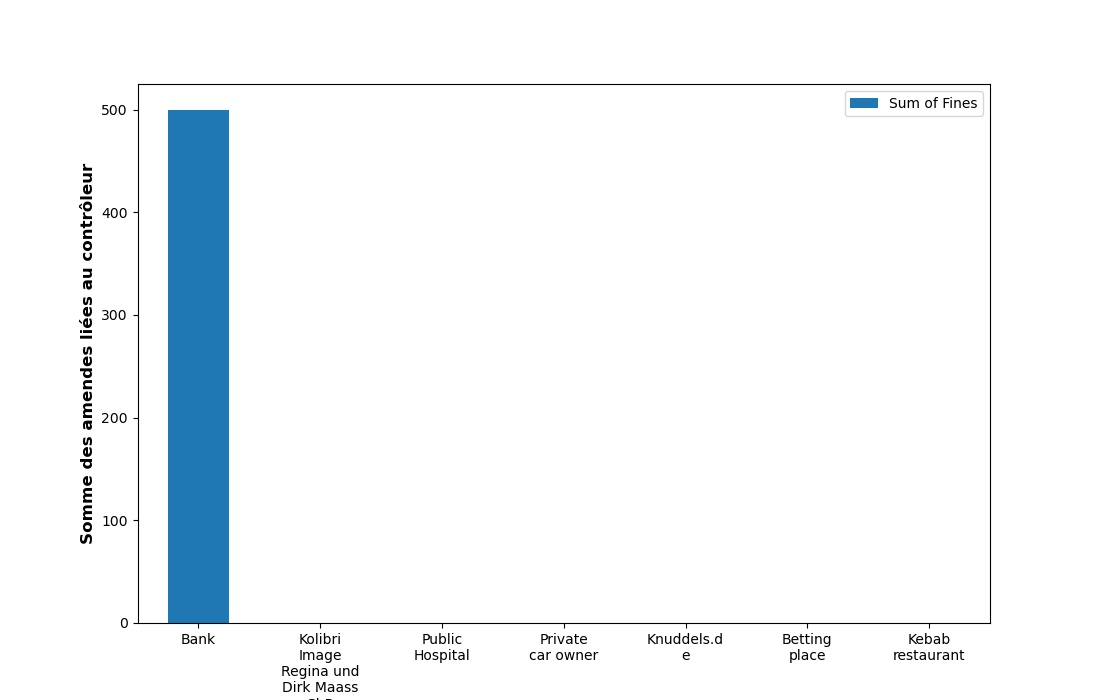
\includegraphics[width=1\linewidth]{graphs/top10_controller_year_fines}
		\caption{Top 10 des entreprises avec le montant le plus élevé d'amendes en 2020}
	 \end{figure}
	
	\end{multicols}


		
	\begin{multicols}{2}
	\begin{figure}
		[H]\centering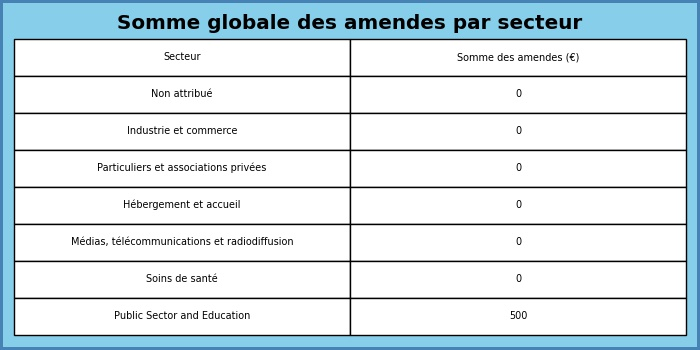
\includegraphics[width=1.0\linewidth]{graphs/sector_data_year_fines}
		\caption{Top 10 des secteurs avec le montant le plus élevé d'amendes2020}
	\end{figure}
	\begin{figure}
		[H]\centering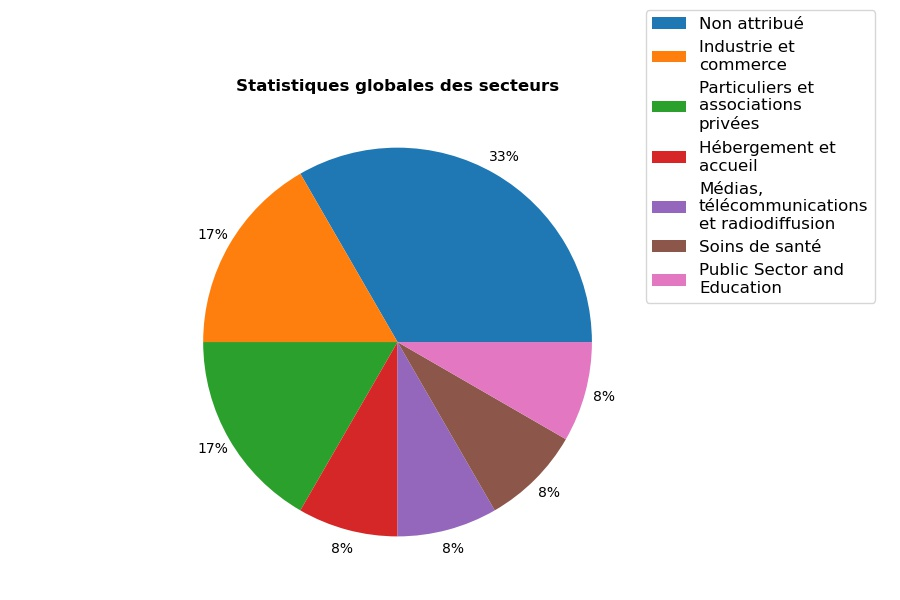
\includegraphics[width=1\linewidth]{graphs/sector_data_year}
		\caption{Top 10 des secteurs avec le montant le plus élevé d'amendes2020}
	 \end{figure}
	
	\end{multicols}

	\begin{multicols}{2}
	\begin{figure}
		[H]\centering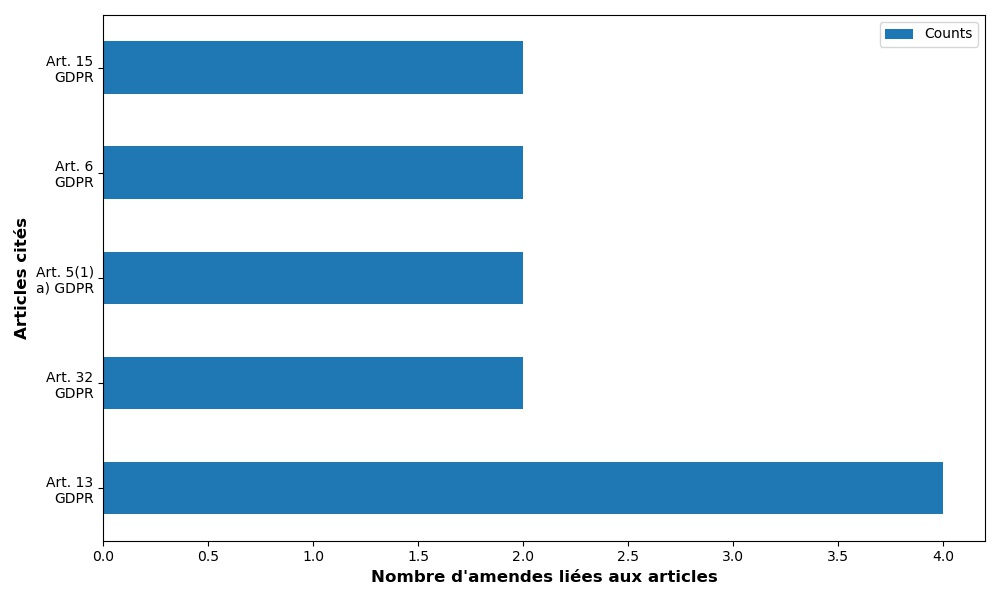
\includegraphics[width=1.0\linewidth]{graphs/top10_quoted_year}
		\caption{Top 5 des articles cités du RGPD avec le plus grand nombre d'amendes en 2020}
	\end{figure}
	\begin{figure}
		[H]\centering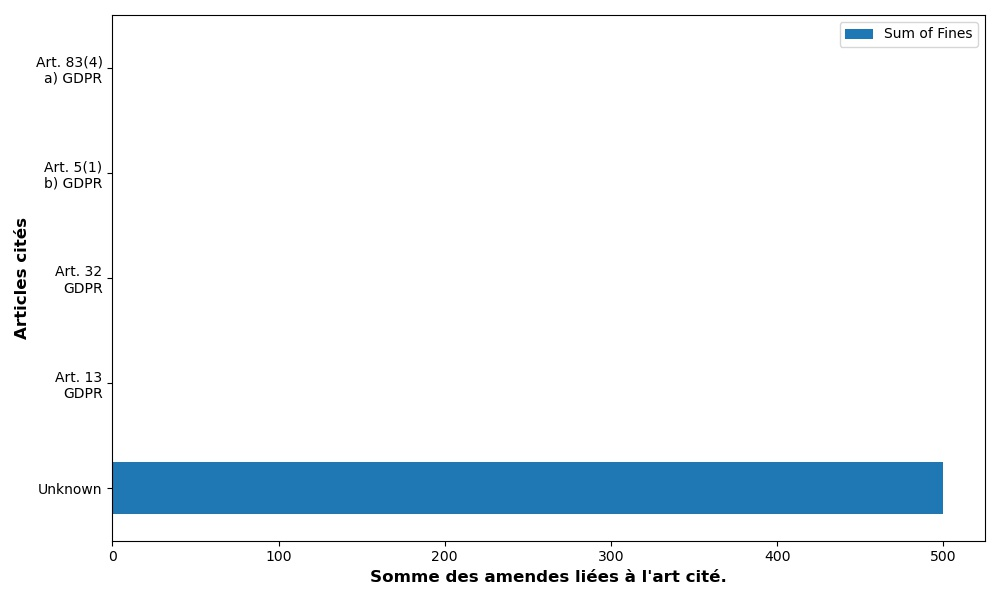
\includegraphics[width=1\linewidth]{graphs/top10_quoted_year_fines}
		\caption{Top 5 des articles  du RGPD avec le montant le plus élevé d'amendes en 2020}
	 \end{figure}
	
	\end{multicols}









\vspace*{\fill}
\textbf{Références:}\\
\href{https://www.enforcementtracker.com}{https://www.enforcementtracker.com}\\
\href{https://brave.com/wp-content/uploads/2020/04/Brave-2020-DPA-Report.pdf}{https://brave.com/wp-content/uploads/2020/04/Brave-2020-DPA-Report.pdf}\\
\href{https://arxiv.org/pdf/2011.00946.pdf}{https://arxiv.org/pdf/2011.00946.pdf}


\end{document}